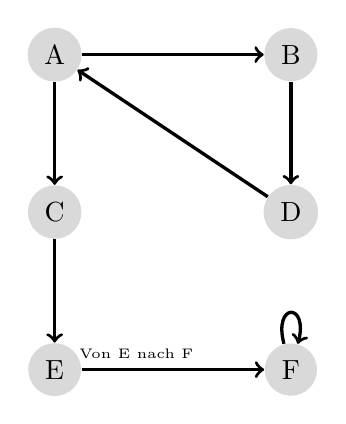
\begin{tikzpicture}
  \node (A) at (0, 4) [circle, fill=gray!30] {A};
  \node (B) at (3, 4) [circle, fill=gray!30] {B};
  \node (C) at (0, 2) [circle, fill=gray!30] {C};
  \node (D) at (3, 2) [circle, fill=gray!30] {D};
  \node (E) at (0, 0) [circle, fill=gray!30] {E};
  \node (F) at (3, 0) [circle, fill=gray!30] {F};

  \draw[->, very thick] (A) to (B);
  \draw[->, very thick] (B) to (D);
  \draw[->, very thick] (D) to (A);
  \draw[->, very thick] (A) to (C);
  \draw[->, very thick] (C) to (E);
  \draw[->, very thick] (E) to node[pos=0.3,above] {\tiny{Von E nach F}} (F);
  \draw[->, very thick] (F) to[loop above] (F);
\end{tikzpicture}
